% \VignetteIndexEntry{Introduction to OLIN}
% \VignetteDepends{OLIN}
% \VignetteKeywords{Expression Analysis, Preprocessing}
% \VignettePackage{OLIN}

\documentclass[a4paper,11pt]{article}
\usepackage{a4wide}
\title{Introduction to OLIN package}
\author{Matthias E. Futschik\\ Institute for Theoretical Biology,  Humboldt-University\\ URL: \textit{http://itb.biologie.hu-berlin.de/$\sim$futschik/software/R/OLIN}}

\usepackage{/usr/lib/R/share/texmf/Sweave}
\begin{document}
\maketitle
\tableofcontents

\section{Overview}
Microarray measurements are affected by a variety of systematic experimental errors 
limiting the accuracy of data produced. 
Two well-known systematic errors for two-colour arrays are    
the so-called intensity-dependent and spatial (location-dependent) dye bias. 
Normalisation aims to correct for systematic errors in microarray data.

The common linear (or global) normalisation method  often fails to correct for dye  bias 
as this bias is usually not linear.  Although non-linear normalisation procedures have been 
able to reduce the systematic errors,
these methods are based on default parameters and leave it to the user to choose ``good'' 
parameters. The optimal adjustment of the normalisation models to the data, however,
can be crucial for the efficiency of the normalisation process \cite{toni}. 

The OLIN (\textit{Optimised Local Intensity-dependent Normalisation})  
R-package includes two normalisation schemes based on iterative  local regression
and model selection. Both  schemes aim to correct for intensity- and location-dependent  dye bias in  microarray data. For model selection (parameter optimisation), generalized cross-validation (GCV) is used. 

Additionally, several procedures to assess the efficiencies of normalisation are implemented
in the package. 

A graphical user interface for OLIN has been implemented in the package OLINgui, that
can be downloaded from the OLIN webpage (\textit{http://itb.biologie.hu-berlin.de/$\sim$futschik/software/R/OLIN}).

%%%%%%%%%%%%%%%%%%%%%%%%%%%%%%%%%%%%%%%%%%%%%%%%%%%%%%%%%%%%%%%%%%%%%%%%%%%%%%%%
%%%%%%%%%%%
\section{Installation requirements}
Following software is required to run the OLIN-package:
\begin{itemize} 
\item  R (> 2.0.0). For installation of R, refer to \textit{http://www.r-project.org}.
\item  R-packages: methods, stats, locfit. For installation of these add-on packages, refer to \textit{http://cran.r-project.org}.
\item Bioconductor packages: Biobase, marray. Refer to \textit{http://www.bioconductor.org} for installation. 
\end{itemize}

If all requirements are fulfilled, the OLIN add-on R-package can be installed. To see how to install add-on R-packages on your computer system, start \textit{R} and type in \textit{help(INSTALL)}.
Optionally, you may use the R-function \textit{install.packages()}. 
Once the OLIN package is installed, you can load the package by 

\begin{Schunk}
\begin{Sinput}
> library(OLIN)
\end{Sinput}
\end{Schunk}



%%%%%%%%%%%%%%%%%%%%%%%%%%%%%%%%%%%%%%%%%%%%%%%%%%%%%%%%%%%%%%%%%%%%%%%%%
\section{Inspection for  intensity-dependent and spatial artifacts}
\label{visu}
Microarray data often contains many systematic errors.
 Such errors have to be identified and removed
 before further data analysis is conducted.  The most basic approach for identification 
 is the visual inspection 
of MA- and MXY-plots. MA-plots display the logged fold change 
($M=log_{2}(Ch2) - log_{2}{Ch1}$)
with respect to the average logged spot intensity  ($A=0.5(log_{2}(Ch1) + log_{2}{Ch2})$).
MXY-plots display $M$ with respect to the corresponding spot location. 
More stringent, but also computationally more expensive,  are statistical tests presented in section \ref{stats}. 


For illustration, we examine a cDNA microarray experiment comparing  gene expression in two colon cancer cell lines (SW480/SW620). The SW480 cell line was derived from a primary tumor, whereas 
the SW620 cell line was cultured from a lymph node metastasis of the same patient.
 Sharing the same genetic background, these cell lines serve as a  model
 of cancer progression~\cite{genomeletters}. The comparison was direct i.e. without using a 
reference sample. cDNA derived from SW480 cells was labeled by Cy3; cDNA derived 
from SW620 was labeled by Cy5. The SW480/620 experiment consisted of four 
technical replicates. The data is stored as object of the class \texttt{marrayRaw} (see
the documentation for the package \texttt{marray}). The average logged spot intensity
$A$ and logged fold changes $M$ can be accessed by using   the slot accessor methods \texttt{maA} and \texttt{maM}, respectively.


First we want to load the data and inspect the spatial distribution of foreground and
background intensities in both channels. This can be done using the  function \texttt{fgbg}
that plots the spatial distribution of fore- and background spot intensities for both channels (figure~\ref{fgbg}):

\begin{Schunk}
\begin{Sinput}
> data(sw)
> fgbg.visu(sw[, 3])
\end{Sinput}
\end{Schunk}

\begin{figure}
\centering
\includegraphics{OLIN-003}
\caption{Foreground and background fluorescence intensities for Cy5-channel (top row) and Cy3-channel (bottom) row.}
\label{fgbg}
\end{figure}

%%%%%%%%%%%%%%%
The  quantity that we are interested in are the (logged) fold-change $M$. To inspect
any existing intensity- or location-dependent bias of $M$, MA- and MXY-lots can be employed.
For MA-lots, the basic \texttt{plot} function can be used (figure~\ref{maplot}). 
MXY-lots can be generated 
by \texttt{mxy.plot}(figure~\ref{mxyplot}). 
Note that the function   \texttt{mxy.plot} assumes the standard array
layout as defined for \textit{marrayRaw/marrayNorm} objects.
  
\begin{Schunk}
\begin{Sinput}
> plot(maA(sw[, 3]), maM(sw[, 3]), xlab = "A", ylab = "M")
\end{Sinput}
\end{Schunk}

%%%%%%%%%%%%%%%%%%%%%%%%%%%%%%%%%%%%%
\begin{figure}[t]
\centering
\includegraphics{OLIN-005}
\caption{MA-plot of SW480/620 array 3}\
\label{maplot}
\end{figure}

%%%%%%%%%%%%%%%%%%%%%%%%%%%%%%%%%%%%%%

\begin{Schunk}
\begin{Sinput}
> mxy.plot(maM(sw)[, 3], Ngc = maNgc(sw), Ngr = maNgr(sw), Nsc = maNsc(sw), 
+     Nsr = maNsr(sw))
\end{Sinput}
\end{Schunk}

%%%%%%%%%%%%%%%%%%%%%%%%%%%%%%%%%%%%%%
\begin{figure}[t]
\centering
\includegraphics{OLIN-007}
\caption{MXY-plot of SW480/620 array 3 with columns and rows as proxies for spatial location}
\label{mxyplot}
\end{figure}
%%%%%%%%%%%%%%%%%%%%%%%%%%%%%%%%%%%%%%

Additionally the distribution of absolute values of $M$ can be displayed. This visualisation
may give an indication whether the span of $M$ is equal across the spatial dimensions of
the array (figure~\ref{mxyabsplot}). 
To plot $abs(M)$, the function \texttt{mxy.abs.plot} can be employed :


\begin{Schunk}
\begin{Sinput}
> data(sw.xy)
> mxy.abs.plot(maM(sw)[, 3], Ngc = maNgc(sw), Ngr = maNgr(sw), 
+     Nsc = maNsc(sw), Nsr = maNsr(sw))
\end{Sinput}
\end{Schunk}

%%%%%%%%%%%%%%%%%%%%%%%%%%%%%
\begin{figure}[t]
\centering
\includegraphics{OLIN-009}
\caption{MXY-plot of absolute logged fold changes}
\label{mxyabsplot}
\end{figure}

%%%%%%%%%%%%%%%%%%%%%%%%%%%%%%%%%%%%%%%%%%%%%%%%%%%%%%%%%%%%

For the two MXY-plots above, the column and row indices were used as proxies for location 
of the spot. We can use, however, the physical spot location as determined by the 
scanner for the MXY plots (if the spots' $X$-and $Y$-coordinates are available.) 
Especially, if the gaps between the blocks printed by distinct pins are large,
this option may give a better physical representation of the array.
Using the function \texttt{mxy2.plot}, such plots can be generated (figure~\ref{mxy2plot}): 

%%%%%%%%%%%%%%%%%%%%%%%%%%%%%%%%%%%%%%%
\begin{Schunk}
\begin{Sinput}
> data(sw.xy)
> mxy2.plot(maM(sw)[, 3], X = sw.xy$X[, 3], Y = sw.xy$Y[, 3], Ngc = maNgc(sw), 
+     Ngr = maNgr(sw), Nsc = maNsc(sw), Nsr = maNsr(sw))
\end{Sinput}
\end{Schunk}

%%%%%%%%%%%%%%%%%%%%%%%%%%%%%%%%%%%%%%%
\begin{figure}[t]
\centering
\includegraphics{OLIN-011}
\caption{MXY plot of SW480/620 array 1}
\label{mxy2plot}
\end{figure}

%%%%%%%%%%%%%%%%%%%%%%%%%%%%%%%%%%%%%%%%%%%%%%%%%%%%%%%%%%%%%%%%
%%%%%%%%%%%%%%%%%%%%%%%%%%%%%%%%%%%%%%%%%%%%%%%%%%%%%%%%%%%%%%%%%%%%%%%%%%%%%%%%%%%%%%%%%%%%%%%%%%

\section{Optimised local intensity-dependent normalisation}
Inspection of the MA- and MXY-plots in the previous section indicated a intensity- and location-dependent dye 
bias. Additionally, the plots show clearly the non-linearity of the biases. To correct for these systematic errors,
 we apply first a local regression of \emph{M} with respect to \emph{A} and spot location \emph{X,Y}.
The residuals of the regression are normalised \emph{M}.This procedure is motivated by the hybridisation model introduced in reference~\cite{toni}.

 The assumption here are: i) Most genes arrayed are not differentially expressed or 
up-and down-regulation is balanced over the range of \emph{A},  ii) the spotting procedure did not generate an spatial accumulation of up- or down-regulated genes in localized areas on the array. 
The validity of both assumptions  should be carefully checked for the data to be normalised. 


The local regression is performed using LOCFIT algorithm which is based on the same 
computational ideas as popular lowess method~\cite{loader,cleveland} .  Required parameters for LOCFIT 
are the smoothing parameter $\alpha$  and the scale parameter(s) \emph{s}
for multi-dimensional regression.
The parameter $\alpha$  specifies the fraction of points that are included in the neighborhood for 
local fitting  and can have a  value between 0 and 1. Larger  values lead to smoother fits.  
The setting of scale parameters s is necessary for a local regression with multiple  
predictor variables. The scale parameters $s$  determine the  amount of smoothing in one direction 
compared to the other directions.   


Choosing accurate regression parameters is crucial for the quality of the normalisation. 
Too large smoothing parameters, for example, lead to a poor fit where local data features are missed
and underfitting occurs.  If the smoothing parameter is too small,  overfitting is produced and
the residuals subsequently underestimated. 
To optimise the parameter setting, two procedures were developed: OLIN and OSLIN. Both methods
are based  on iterative local regression and parameter selection by GCV.
 They aim to correct for systematic errors linked with spot intensity and location. A detailed mathematical description can be found in reference~\cite{toni}.


\subsection{OLIN}
The OLIN (and OSLIN) are implemented in R by the function \texttt{olin}:

\begin{quote}
\texttt{olin(object,X,Y,alpha,iter,OSLIN,scale,weights,genepix,bg.corr,...)}
\end{quote}


\noindent The input arguments are  as follows:
           \begin{description}
           \item[object] Object of class \emph{marrayRaw} or \emph{marrayNorm} containing 
                         data of the microarray experiment such as spot intensities and array layout
                         for a batch of microarrays.
                         To generate such an object, see the \emph{marryClasses} documentation.
           \item[X]      matrix with x-coordinates of spots. Each column corresponds to one array in the batch. The location is spots detected by scanner
                         is usually 
                         found in the output file program of  the scanning program. 
                          If X=NA, the spotted columns on the  array are used as proxies for the location in x-direction (\emph{default})
           \item[Y] matrix with y-coordinates of spots. If Y=NA, spotted rows on array are used
            as proxies for the location in y-direction (\emph{default}).
           \item[alpha] Vector of $\alpha$  parameters that are tested in the GCV procedure. The $\alpha$  parameter 
                  defines the smoothness of fit.  The default vector is \texttt{seq(0.05,1,0.1)}.
           \item[iter] Number of iterations in the OLIN or OSLIN procedure. The default value is 3. 
           \item[OSLIN] If OSLIN =TRUE, a subsequent optimised scaling of the range of M across the array
                        is performed.
                         The default value is \emph{FALSE}, i.e. OLIN is performed. 
           \item[scale] Vector of scale parameters \emph{s} that are tested in a GCV procedure. 
                    This  allows  a different amount of smoothing in Y-direction compared 
                    to smoothing in X-direction. The default values of \emph{s} are 
                    \texttt{c(0.05,0.1,0.5,1,2,10,20))}.
           \item[weights] Matrix of prior weights of spots for the regression procedures.
                          Spots can be excluded to be used
                          for the local regression by assigning them to zero.  
                          If the weight matrix include negative values, these will be
	                   set to zero.\\
                          For the weights, the weight matrix stored 
                          in the \texttt{maW} slot of  \emph{marrayRaw} objects can be used 
                           (\texttt{weights=maW(object)}). Defaults is \texttt{NA} resulting
                          in uniform weigths of all spots. 
	\item[genepix]{If \texttt{genepix} is set to 
			\texttt{TRUE},  spot weights equal zero or larger are set
			to one for the local regression whereas negative
			spot with negative weights are not used   for the
			regression. The argument \texttt{genepix} should
			be set to \texttt{TRUE}, if
			\texttt{weights=maW(object)} is set and  spot
			quality weights derived by GenePix are stored in
			\texttt{maW(object)}.}
            \item[bg.corr] backcorrection method (for \emph{marrayRaw} objects)  :
			\emph{none} - no background correction, \emph{sub} 
                          - simple background subtraction (default), 
            \emph{movingmin} -  background intensities are first averaged over 3x3 grids
  of neighbouring spots and subsequently substracte, 
 \emph{minimum} - zero or negative intensities after background
        correction are set equal to half the minimum of positive
        corrected intensities, \emph{edwards}-  background correction based on  log-linear
       interpolation, or \emph{normexp}-  background correction based on fitting
       procedure. For further details and references, please refer to to the  help page
of \texttt{backgroundCorrect2} of the \emph{OLIN} package or \texttt{backgroundCorrect} of the \emph{limma} package.
 

          \item[...] Further arguments passed to the  \texttt{locfit} function.	
      \end{description}


For illustration, we apply the OLIN scheme to normalise the third array of the SW480/620 data set. 
(Note that the function is not restricted to single slide normalisation but normalises all arrays
in the given \emph{marray} object.)

\begin{Schunk}
\begin{Sinput}
> norm.olin <- olin(sw[, 3], X = sw.xy$X[, 3], Y = sw.xy$Y[, 3])
\end{Sinput}
\end{Schunk}

Inspection of the MA- and MXY-plot indicated that OLIN  was able to correct for the  
intensity- as well as  the  location-dependent dye bias. The
 residuals are well  balanced around zero in the MA-plot (figure~\ref{maolin}).
Similarly, spatial bias is no longer apparent (figure~\ref{mxyolin}).
Spots with positive and negative log ratio M were evenly distributed across the slide. 
The statistical tests
applied in the next section will confirm  these findings. 

\begin{Schunk}
\begin{Sinput}
> plot(maA(norm.olin), maM(norm.olin), main = "OLIN", pch = ".")
> mxy.plot(maM(norm.olin), Ngc = maNgc(norm.olin), Ngr = maNgr(norm.olin), 
+     Nsc = maNsc(norm.olin), Nsr = maNsr(norm.olin), main = "OLIN")
\end{Sinput}
\end{Schunk}


%%%%%%%%%%%%%%%%

\begin{figure}[t]
\centering
\includegraphics{OLIN-014}
\caption{MA-plot of array normalized by  OLIN }
\label{maolin}
\end{figure}

%%%%%%%%%%%%%%%%%%%%%%%%%%%%


\begin{figure}
\centering
\includegraphics{OLIN-015}
\caption{MXY-plot of array normalized by  OLIN }
\label{mxyolin}
\end{figure}
%%%%%%%%%%%%%%%%%%%%%%%%%%%%%%%%%%%%%


OLIN is based on an iterative procedure. In most cases, we found
that two or three iterations are already sufficient for normalisation (figure~\ref{iter}).   


\begin{Schunk}
\begin{Sinput}
> norm.olin.1 <- olin(sw[, 3], X = sw.xy$X[, 3], Y = sw.xy$Y[, 
+     3], iter = 1)
> norm.olin.2 <- olin(norm.olin.1, X = sw.xy$X[, 3], Y = sw.xy$Y[, 
+     3], iter = 1)
> norm.olin.3 <- olin(norm.olin.2, X = sw.xy$X[, 3], Y = sw.xy$Y[, 
+     3], iter = 1)
> M <- cbind(maM(sw)[, 3], maM(norm.olin.1), maM(norm.olin.2), 
+     maM(norm.olin.3))
> pairs(M, labels = c("raw", "1.Iter.", "2.Iter.", "3.Iter."))
\end{Sinput}
\end{Schunk}


\begin{figure}[t]
\centering
\resizebox{0.8\textwidth}{!}{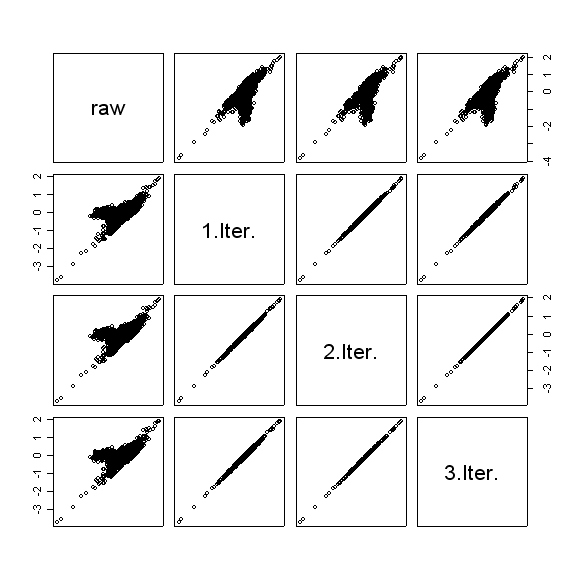
\includegraphics{scatter.png}}
\caption{Convergence of iterative normalisation }
\label{iter}
\end{figure}

%%%%%%%%%%%%%%%%%%%%%%%%%%%%%%%%%%%%%%%%%%%%%%%%%%%%%%%%



%%%%%%%%%%%%%%%%%%%%%%%%%%%%%%%
\subsection{OSLIN} 
If we can assume that the variability of log ratios M should be equal across the array,
 local scaling of \emph{M} can be performed. As in the previous section, the validity of these assumptions
 has to be carefully checked for each experiment analyzed. The underlying requirement is again random 
spotting of arrayed genes. To apply OSLIN:

\begin{Schunk}
\begin{Sinput}
> norm.oslin <- olin(sw[, 3], X = sw.xy$X[, 3], Y = sw.xy$Y[, 3], 
+     alpha = c(0.1, 1, 0.1), OSLIN = TRUE)
\end{Sinput}
\end{Schunk}

The local scaling factors are  derived by optimized local regression of the absolute log ratio M. 
The range of regression  parameters tested by GCV is [0.1,1] for smoothing parameter. 
The resulting MA- and MXY-plots for slide 3 are presented in figures~\ref{maoslin} and \ref{mxyoslin}.. 
The variability of log ratios \emph{M} appears to be even across the array.

%%%%%%%%%%%%%%%%%%%%%%%%%%

\begin{Schunk}
\begin{Sinput}
> plot(maA(norm.oslin), maM(norm.oslin), main = "OSLIN", pch = ".")
> mxy.plot(maM(norm.oslin), Ngc = maNgc(norm.oslin), Ngr = maNgr(norm.oslin), 
+     Nsc = maNsc(norm.oslin), Nsr = maNsr(norm.oslin), main = "OSLIN")
\end{Sinput}
\end{Schunk}


%%%%%%%%%%%%%%%%

\begin{figure}[t]
\centering
\includegraphics{OLIN-019}
\caption{MA-plot of array normalized by  OSLIN }
\label{maoslin}
\end{figure}

%%%%%%%%%%%%%%%%%%%%%%%%%%%%
The \emph{weights} argument can be used for two purposes. First, it can be 
to exclude a set of spots (such as control spots)  to be used  for local regression. Second, it can be used 
to base the regression on a selected set of genes assumed to be not differentially expressed (\emph{house-keeping
genes}).  
If the normalisation should be based on such a set, weights can be used for local regression. 
In this case, all weights should be  set to zero except for
the house-keeping genes for which weights are set to one. In order to achieve a reliable regression, it is important, however, that there is a sufficient number of house-keeping genes that  cover the whole expression range
and are spotted accross the whole array.

%%%%%%%%%%%%%%%%%%%%%%%%%


\begin{figure}[t]
\centering
\includegraphics{OLIN-020}
\caption{MXY-plot of array normalized by  OSLIN }
\label{mxyoslin}
\end{figure}
%%%%%%%%%%%%%%%%%%%%%%%%%%%%%%%%%%%%%

Note that OLIN and OSLIN
are sensitive to violations of the assumptions that
 most genes are not differentially expressed (or up- and down-regulation
is balanced) and that genes are randomly spotted across the array. 
If these assumptions are not valid, local
regression can lead to an underestimation of differential expression.  
In this context,  OSLIN is especially sensitive in its performance. However, the
sensitivity can be decreased if the minimal smooting parameter \texttt{alpha} (default value: 0.05)
 is set to larger values. 
 

It is also important to note that OLIN/OSLIN is fairly efficient in removing intensity- and spatial-dependent dye bias, so that normalised  data will look quite "good" after normalisation independently of the true underlying data quality. Normalisation by local regression assumes smoothness of bias. Therefore, localised artifacts such as scratches, edge effects or bubbles should be avoided. Spots of these areas should be flagged (before normalization is applied) to ensure data integrity. To stringently detect artifacts, the OLIN functions \texttt{fdr.int, fdr.int2, fdr.spatial,fdr.spatial2, 
p.int, p.int2, p.spatial} and \texttt{p.spatial2} can be used. 
Flagging of the data spots in regions of intensity- or location-dependent bias can be performed 
by \texttt{sig.mask}. For an example of such an flagging or masking procedure, 
see the help page of \texttt{sig.mask}.


\section{Scaling between arrays of a batch}
OLIN and OSLIN adjust log ratio \emph{M} of an array independently of other arrays.
A further reduction  of variation within experiments may be achieved by
additional scaling of M between arrays \cite{yang}. This procedure is frequently
also termed 'between-array normalisation' in contrast to 'within-array normalisation'
as for example performed by O(S)LIN. The log ratios of \emph{M} will be adjusted in different
arrays to achieve a similar overall distribution of \emph{M}.

However, it assumes that the overall scale of M is the same (or at least similar)
in the different arrays to be scaled. This should be  carefully checked. Differences in the 
overall scale of \emph{M} may indicated e.g. changes in hybridisation conditions or mRNA quality.
Caution should also be taken in the interpretation of results for arrays
hybridised with  biologically divergent samples, if between-array  scaling is applied.


Between-array scaling is implemented in the \emph{OLIN} package through function \texttt{bas}.
Three different scaling procedures are supported: 
\begin{enumerate}
\item  arrays are scaled to have the same variance as calculated by
\texttt{var},
\item  arrays are scaled to have the same median absolute deviation calculated by \texttt{mad}
\item arrays are scaled to have  equal values of quantiles. 
\end{enumerate}

For illustration, we apply the first scaling procedure to  OLIN-adjusted SW480/620 data consisting of four
replicate array (figures~\ref{disolin},ref{disbas}):

 
\begin{Schunk}
\begin{Sinput}
> data(sw.olin)
> col <- c("red", "blue", "green", "orange")
> M <- maM(sw.olin)
> plot(density(M[, 4]), col = col[4], xlim = c(-2, 2))
> for (i in 1:3) {
+     lines(density(M[, i]), col = col[i])
+ }
> sw.olin.s <- bas(sw.olin, mode = "var")
> M <- maM(sw.olin.s)
> plot(density(M[, 4]), col = col[4], xlim = c(-2, 2))
> for (i in 1:3) {
+     lines(density(M[, i]), col = col[i])
+ }
\end{Sinput}
\end{Schunk}


%%%%%%%%%%%%%%%%

\begin{figure}[t]
\centering
\includegraphics{OLIN-022}
\caption{Distribution of M for SW480/620 arrays after OLIN  }
\label{disolin}
\end{figure}


\begin{figure}[t]
\centering
\includegraphics{OLIN-023}
\caption{Distribution of M for SW480/620 arrays after OLIN and between-array scaling}
\label{disbas}
\end{figure}

%%%%%%%



 

%%%%%%%%%%%%%%%%%%%%%%%%%%%%%%%%%%%%%%%%%%%%%%%%%%%%%%%%%%%%%%%%%%%%%%%%%%%%%%%%%%%%%%%%%%%%%%%%%%%%%%%%%
%%%%%%%%%%%%%%%%%%%%%%%%%%%%%%%%%%%%%%%%%%%%%%%%%%%

%%%%%%%%%
\section{Statistical assessment of efficiency of normalisation}
\label{stats}
An important criterion for the quality of normalisation is its efficiency in 
removing systematic errors. Although visual inspection might readily reveal prominent
artifacts in the microarray data (as shown in section~\ref{visu}), it does not allow for their stringent 
detection. To overcome this limitation, several methods for statistical detection of 
systematic errors were implemented in the OLIN package. They might be especially valuable
for the comparison of the efficiency of different normalisation methods. They also might 
be helpful for newcomers in the field of microarray data analysis, since they can assist the
detection of artifacts and may help to improve the experimental procedures.

A simple method to detect intensity- or location-dependent  bias is to calculate the 
correlation between the log ratio \emph{M} of a spot and the average \emph{M} in the spot's 
neighbourhood ~\cite{jo}. A neighourhood on the intensity scale can be defined by a symmetrical
window of size (2*$delta$ + 1) around the spot. A correlation of zero can be expected assuming
the log ratios are uncorrelated. In contrast, a large positive correlation indicates intensity-dependent
 bias.

\begin{Schunk}
\begin{Sinput}
> A <- maA(sw[, 3])
> M <- maM(sw[, 3])
> Mav <- ma.vector(A, M, av = "median", delta = 50)
> cor(Mav, M, use = "pairwise.complete.obs")
\end{Sinput}
\begin{Soutput}
          [,1]
[1,] 0.6416701
\end{Soutput}
\end{Schunk}

Similarly, the location-dependent bias can be assessed: 

\begin{Schunk}
\begin{Sinput}
> MM <- v2m(maM(sw)[, 3], Ngc = maNgc(sw), Ngr = maNgr(sw), Nsc = maNsc(sw), 
+     Nsr = maNsr(sw), visu = FALSE)
> MMav <- ma.matrix(MM, av = "median", delta = 2, edgeNA = FALSE)
> Mav <- m2v(MMav, Ngc = maNgc(sw), Ngr = maNgr(sw), Nsc = maNsc(sw), 
+     Nsr = maNsr(sw), visu = FALSE)
> cor(Mav, M, use = "pairwise.complete.obs")
\end{Sinput}
\begin{Soutput}
          [,1]
[1,] 0.4377952
\end{Soutput}
\end{Schunk}

Although correlation analysis can be readily applied, it  cannot 
deliver localization of experimental bias in the data. 
To detect areas of bias in the microarray data, alternative methods can be applied. 

The OLIN package contains two four models. The first model (\texttt{anovaint}) can be used
to assess intensity-dependent bias. For this task, the A-scale is divided into \emph{N} intervals
containing equal number of spots. The null hypothesis tested is the equality of the means of \emph{M} for the different intervals.  The input argument \texttt{index} indicates which array stored in object \emph{sw}
 should
be examined. 
The function \texttt{anovaint}  is a wrapper around the core function \texttt{lm}. 
The output of  \texttt{anovaint} equals \texttt{summery(lm)}.

\begin{Schunk}
\begin{Sinput}
> print(anovaint(sw, index = 3, N = 10))
\end{Sinput}
\begin{Soutput}
Call:
lm(formula = Mo ~ intensityint - 1)

Residuals:
     Min       1Q   Median       3Q      Max 
-4.06150 -0.18971  0.01900  0.23877  1.77781 

Coefficients:
               Estimate Std. Error t value Pr(>|t|)    
intensityint1  -0.86456    0.01856 -46.578  < 2e-16 ***
intensityint2  -0.11228    0.01856  -6.049 1.58e-09 ***
intensityint3   0.01868    0.01856   1.006 0.314355    
intensityint4   0.06458    0.01856   3.479 0.000508 ***
intensityint5   0.16762    0.01856   9.030  < 2e-16 ***
intensityint6   0.19606    0.01856  10.563  < 2e-16 ***
intensityint7   0.25546    0.01856  13.763  < 2e-16 ***
intensityint8   0.21835    0.01856  11.763  < 2e-16 ***
intensityint9   0.24910    0.01856  13.420  < 2e-16 ***
intensityint10  0.21253    0.01869  11.369  < 2e-16 ***
---
Signif. codes:  0 `***' 0.001 `**' 0.01 `*' 0.05 `.' 0.1 ` ' 1 

Residual standard error: 0.3818 on 4214 degrees of freedom
Multiple R-Squared: 0.4198,	Adjusted R-squared: 0.4185 
F-statistic: 304.9 on 10 and 4214 DF,  p-value: < 2.2e-16 
\end{Soutput}
\end{Schunk}

\begin{Schunk}
\begin{Sinput}
> data(sw.olin)
> print(anovaint(sw.olin, index = 3, N = 10))
\end{Sinput}
\begin{Soutput}
Call:
lm(formula = Mo ~ intensityint - 1)

Residuals:
     Min       1Q   Median       3Q      Max 
-3.59972 -0.12592  0.02501  0.16397  1.86714 

Coefficients:
                 Estimate Std. Error t value Pr(>|t|)
intensityint1  -0.0049581  0.0153753  -0.322    0.747
intensityint2   0.0085228  0.0153753   0.554    0.579
intensityint3   0.0100288  0.0153753   0.652    0.514
intensityint4   0.0092998  0.0153753   0.605    0.545
intensityint5  -0.0006992  0.0153753  -0.045    0.964
intensityint6  -0.0047550  0.0153753  -0.309    0.757
intensityint7  -0.0156696  0.0153753  -1.019    0.308
intensityint8  -0.0051047  0.0153753  -0.332    0.740
intensityint9   0.0030058  0.0153753   0.195    0.845
intensityint10  0.0005948  0.0154856   0.038    0.969

Residual standard error: 0.3162 on 4214 degrees of freedom
Multiple R-Squared: 0.0005903,	Adjusted R-squared: -0.001781 
F-statistic: 0.2489 on 10 and 4214 DF,  p-value: 0.991 
\end{Soutput}
\end{Schunk}


Similarly, the location-dependent bias can be examined by an ANOVA model implemented as
\texttt{anovaspatial}. The array is divided into (xN x yN) rectangular blocks.   
The null hypothesis tested is the equality of the means of \emph{M} for the different blocks.  
The function \texttt{anovaspatial} is a wrapper around functipn \texttt{lm}. The output
is the summary of \texttt{lm} (which is suppressed in following examples).
Additionally,  \texttt{anovaspatial} allows for visualisation of the results (see figure
~\ref{anova} and \ref{anovaolin}.) The figures display the log10-transformed p-values
as derived in the block-wise \textit{t}-tests. Note that the differences in scales.   


\begin{Schunk}
\begin{Sinput}
> anovaspatial(sw, index = 3, xN = 8, yN = 8, visu = TRUE)
\end{Sinput}
\end{Schunk}

\begin{Schunk}
\begin{Sinput}
> anovaspatial(sw.olin, index = 3, xN = 8, yN = 8, visu = TRUE)
\end{Sinput}
\end{Schunk}

\begin{figure}[t]
\centering
\includegraphics{OLIN-030}
\caption{ANOVA for raw data}
\label{anova}
\end{figure}

\begin{figure}[t]
\centering
\includegraphics{OLIN-031}
\caption{ANOVA for normalised data}
\label{anovaolin}
\end{figure}


Additionally, simple one-factorial ANOVA 
models were implemented to test microarray data for  pin- and plate-dependent
bias. Testing for pin bias by \texttt{anovapin} is similar to testing for spatial 
bias by \texttt{anovaspatial}. The factors in \texttt{anovapin} are the pin indices.
The null hypothesis is the equality of the means of \emph{M} for the different pins.
In the same manner, it can be tested if there is a significant variation of \emph{M}
due to the use of distinct microtiter plate for spotting. An ANOVA model for this
task is implemented in function \texttt{anovaplate}.In this case, the null hypothesis 
is the equality of the means of \emph{M} for the different plates.

\begin{Schunk}
\begin{Sinput}
> print(anovapin(sw.olin, index = 3))
\end{Sinput}
\begin{Soutput}
Call:
lm(formula = M ~ pin - 1)

Residuals:
     Min       1Q   Median       3Q      Max 
-3.60963 -0.12436  0.02528  0.16397  1.86083 

Coefficients:
        Estimate Std. Error t value Pr(>|t|)
pin1   0.0057223  0.0194744   0.294    0.769
pin2   0.0009404  0.0194744   0.048    0.961
pin3  -0.0011836  0.0194744  -0.061    0.952
pin4  -0.0002191  0.0194744  -0.011    0.991
pin5  -0.0077155  0.0194744  -0.396    0.692
pin6  -0.0051030  0.0194744  -0.262    0.793
pin7  -0.0077761  0.0194744  -0.399    0.690
pin8   0.0144356  0.0194744   0.741    0.459
pin9   0.0005014  0.0194744   0.026    0.979
pin10  0.0015559  0.0194744   0.080    0.936
pin11  0.0184692  0.0194744   0.948    0.343
pin12 -0.0047442  0.0194744  -0.244    0.808
pin13  0.0051594  0.0194744   0.265    0.791
pin14 -0.0087071  0.0194744  -0.447    0.655
pin15  0.0068432  0.0194744   0.351    0.725
pin16 -0.0177670  0.0194744  -0.912    0.362

Residual standard error: 0.3164 on 4208 degrees of freedom
Multiple R-Squared: 0.0007643,	Adjusted R-squared: -0.003035 
F-statistic: 0.2012 on 16 and 4208 DF,  p-value: 0.9997 
\end{Soutput}
\end{Schunk}


\begin{Schunk}
\begin{Sinput}
> print(anovaplate(sw.olin, index = 3))
\end{Sinput}
\begin{Soutput}
Call:
lm(formula = M ~ plate - 1)

Residuals:
     Min       1Q   Median       3Q      Max 
-3.59872 -0.12780  0.02606  0.16583  1.84665 

Coefficients:
          Estimate Std. Error t value Pr(>|t|)  
plate1  -0.0226044  0.0161246  -1.402    0.161  
plate2   0.0287166  0.0161246   1.781    0.075 .
plate3  -0.0057500  0.0161246  -0.357    0.721  
plate4   0.0018882  0.0161246   0.117    0.907  
plate5  -0.0125836  0.0161246  -0.780    0.435  
plate6  -0.0015375  0.0161246  -0.095    0.924  
plate7   0.0003773  0.0161246   0.023    0.981  
plate8  -0.0128983  0.0161246  -0.800    0.424  
plate9   0.0157338  0.0161246   0.976    0.329  
plate10 -0.0134014  0.0161246  -0.831    0.406  
plate11  0.0223422  0.0161246   1.386    0.166  
---
Signif. codes:  0 `***' 0.001 `**' 0.01 `*' 0.05 `.' 0.1 ` ' 1 

Residual standard error: 0.316 on 4213 degrees of freedom
Multiple R-Squared: 0.002391,	Adjusted R-squared: -0.0002133 
F-statistic: 0.9181 on 11 and 4213 DF,  p-value: 0.5216 
\end{Soutput}
\end{Schunk}


ANOVA methods assume normality of the analysed data. This, however, may not be the
general case for microarray data. To relax this restriction, permutation tests can be
applied. Permutation (or randomization) tests have the advantage that a particular data 
distribution is not assumed. They rely solely on the observed data examples and can be 
applied with a variety of test statistics. A major restriction, however, is that 
permutation tests are computationally very intensive.
Generally, such tests are not used in interactive mode but are performed in batch-mode. 


Four permutation tests procedures were implemented in the OLIN package. 
The functions \texttt{fdr.int}  and \texttt{p.int} assess intensity-dependent
bias. The functions \texttt{fdr.spatial} and \texttt{p.spatial} assess location-dependent
bias. The basic procedure is similar for all four functions.
First, a (intensity or location)  neighbourhood of spots is defined similarly to the procedure
we used for the correlation analysis .  Next, a test statistic is constructed by calculating
 the \emph{median} or \emph{mean} of \emph{M} the  spot's  neighbourhood of chosen size.
 An empirical distribution of the test statistic $\bar{M}$ is 
then produced  based on random permutations of the
data. Comparing  $\bar{M}$ of the original data with the empirical distribution, the significance 
of observing  $\bar{M}$ is derived. (Note that a rather low number of random permutations was chosen
to avoid time-consuming calculations here. Generally, however, a larger number should be chosen.)  

%%%%%%%%%%%%%%%%%%%%%%%%%%%%%%%%%%%%%%

The functions \texttt{fdr.int}, \texttt{p.int}, \texttt{fdr.spatial} and  \texttt{p.spatial}
perform two one-sided random permutation tests. The result can be visualised by 
the plotting functions \texttt{sigint.plot} and \texttt{sigxy.plot}. 
The significance of a spot neighbourhood with large positive deviations of $\bar{M}$ is 
displayed in red along the A-scale or across the spatial dimensions of the array. 
Correspondingly, the significance of spot neighbourhood with large negative 
deviations of  $\bar{M}$ are displayed in green.  


\begin{Schunk}
\begin{Sinput}
> FDR <- fdr.int(maA(sw)[, 3], maM(sw)[, 3], delta = 50, N = 10, 
+     av = "median")
> sigint.plot(maA(sw)[, 3], maM(sw)[, 3], FDR$FDRp, FDR$FDRn, c(-5, 
+     -5))
\end{Sinput}
\end{Schunk}



\begin{figure}[t]
\centering
\includegraphics{OLIN-035}
\caption{MA-plot and FDRs of  intensity-dependent bias for raw data }
\label{fdrintraw}
\end{figure}



\begin{Schunk}
\begin{Sinput}
> data(sw.olin)
> FDR <- fdr.int(maA(sw.olin)[, 3], maM(sw.olin)[, 3], delta = 50, 
+     N = 10, av = "median")
> sigint.plot(maA(sw.olin)[, 3], maM(sw.olin)[, 3], FDR$FDRp, FDR$FDRn, 
+     c(-5, -5))
\end{Sinput}
\end{Schunk}



\begin{figure}
\centering
\includegraphics{OLIN-037}
\caption{MA-plot and FDRs of  intensity-dependent bias for data normalised by OLIN }
\label{fdrintolin}
\end{figure}

For slide 3, an significant intensity-dependent bias towards channel 2 (Cy3)
was detected for low spot intensities, whereas high-intensity spots are biased
towards channel 2 (figure~\ref{fdrintraw}). After OLIN normalisation, no significant intensity-dependent
bias is apparent (figure~\ref{fdrintolin}). A similar result can be found for the 
removal of location-dependent bias by OLIN (figure~\ref{fdrspatialraw} and \ref{fdrspatialolin}).

%%%%%%%%%%%%%%%%%%%%%%%%%%

\begin{Schunk}
\begin{Sinput}
> M <- v2m(maM(sw)[, 3], Ngc = maNgc(sw), Ngr = maNgr(sw), Nsc = maNsc(sw), 
+     Nsr = maNsr(sw), main = "MXY plot of SW-array 1")
> FDR <- fdr.spatial(M, delta = 2, N = 10, av = "median", edgeNA = TRUE)
> sigxy.plot(FDR$FDRp, FDR$FDRn, color.lim = c(-5, 5), main = "FDR")
\end{Sinput}
\end{Schunk}




\begin{figure}[t]
\centering
\includegraphics{OLIN-039}
\caption{FDR of location-dependent bias for raw data }
\label{fdrspatialraw}
\end{figure}


\begin{Schunk}
\begin{Sinput}
> M <- v2m(maM(sw.olin)[, 3], Ngc = maNgc(sw.olin), Ngr = maNgr(sw.olin), 
+     Nsc = maNsc(sw.olin), Nsr = maNsr(sw.olin), main = "MXY plot of SW-array 1")
> FDR <- fdr.spatial(M, delta = 2, N = 10, av = "median", edgeNA = TRUE)
> sigxy.plot(FDR$FDRp, FDR$FDRn, color.lim = c(-5, 5), main = "FDR")
\end{Sinput}
\end{Schunk}


\begin{figure}
\centering
\includegraphics{OLIN-041}
\caption{FDR of location-dependent bias for data normalised by OLIN}
\label{fdrspatialolin}
\end{figure}


 
Fold changes should be treated with care if the corresponding spots have significantly biased 
neighborhoods even after normalisation. 


The functions \texttt{fdr.int} and \texttt{fdr.spatial} assess the significance of dye bias using the false discovery
rate whereas the related  functions \texttt{p.int} and \texttt{p.spatial} produce (adjusted) p-values.
Another difference between the functions is the procedure to generate random permutation.
The function \texttt{fdr.int} and \texttt{fdr.spatial} are based on re-sampling without replacement,
whereas  \texttt{p.int} and \texttt{p.spatial} are based on re-sampling with replacement.  
A more detailed description of the permutation tests can be found in the \textit{help}-pages of these functions.

Finally, a second set of functions  (\texttt{fdr.int2, p.int2, fdr.spatial2, p.spatial2, sigint.plot2,sigxy.plot2} has been introduced for the present version of the OLIN package. Their functionality is the same as for the first set (i.e. \texttt{fdr.int, p.int,...}). However, the input arguments  and output objects of the functions  may differ (see the  relevant \textit{help}). Both sets will be merged based on S4-style functions in future versions.



%BIBLIOGRAPHY
\begin{thebibliography}{99}
\bibitem{toni} M.Futschik and T. Crompton (2004) Model selection and efficiency testing for normalisation of cDNA microarray data, \emph{Genome Biology}, 5:R60  
\bibitem{genomeletters} M. Futschik, A.Jeffs, S.Pattison, N.Kasabov, M.Sullivan, A.Merrie and A.Reeve (2002) Gene expression profiling of metastatic and non-metastatic colorectal cancer cell-lines,  \emph{Genome Letters}, 1(1) , 26-34
\bibitem{loader} C. Loader (1999) Local regression and likelihood, Springer, New York
\bibitem{cleveland} WS Cleveland (1979) Robust locally weighted regression and smoothing scatterplots,
\emph{J Am Stat Ass}, 74, 829-836
\bibitem{jo} J. Schuchhardt, D. Beule, A. Malik, E. Wolski, H. Eickhoff, H. Lehrach and H.Herzel (2000)
Normalization strategies for cDNA microarrays. \emph{Nucleic Acid Research} 28:e47
\bibitem{yang} Y. H. Yang, S. Dudoit, P. Luu, D. M. Lin, V. Peng, J. Ngai, and T.
     P. Speed (2002). Normalization for cDNA microarray data: a robust
     composite method addressing single and multiple slide systematic
     variation. \emph{Nucleic Acids Research}, Vol. 30, No. 4.
 


\end{thebibliography}

\end{document}

